\subsection{Space Debris}
The Space had been a virgin environment until the middle of the twentieth century. However, it has already been exploited by humanity. During the last sixty years many space research centers –such as NASA, ESA or ROSCOSMOS- have been sending rockets and satellites to explore and understand its foreign environment without thinking on the consequences it could have. Fortunately, at the twenty-first century the concern about space debris has appears. Due to this fact, all those space research centers have begun to develop end-of-life strategies for all the missions that generate debris to restrict its lifetime. 
\newline
\newline
The term Space Debris implicates all man-made objects that are orbiting with no human control. The problem arises from the fact that depending on the orbital parameters this space stuff is subject to more or less perturbations from either the Earth, the Moon, the Sun or the atmospherically drag and, after their operability’s death, they might never disappear or completely disintegrate. As the quantity of space debris is huge and varied, they have been classified in four categories: fragmentation debris, non-functional spacecraft, rocket bodies and mission related debris. 
\newline
\newline
\begin{figure}
\centering 
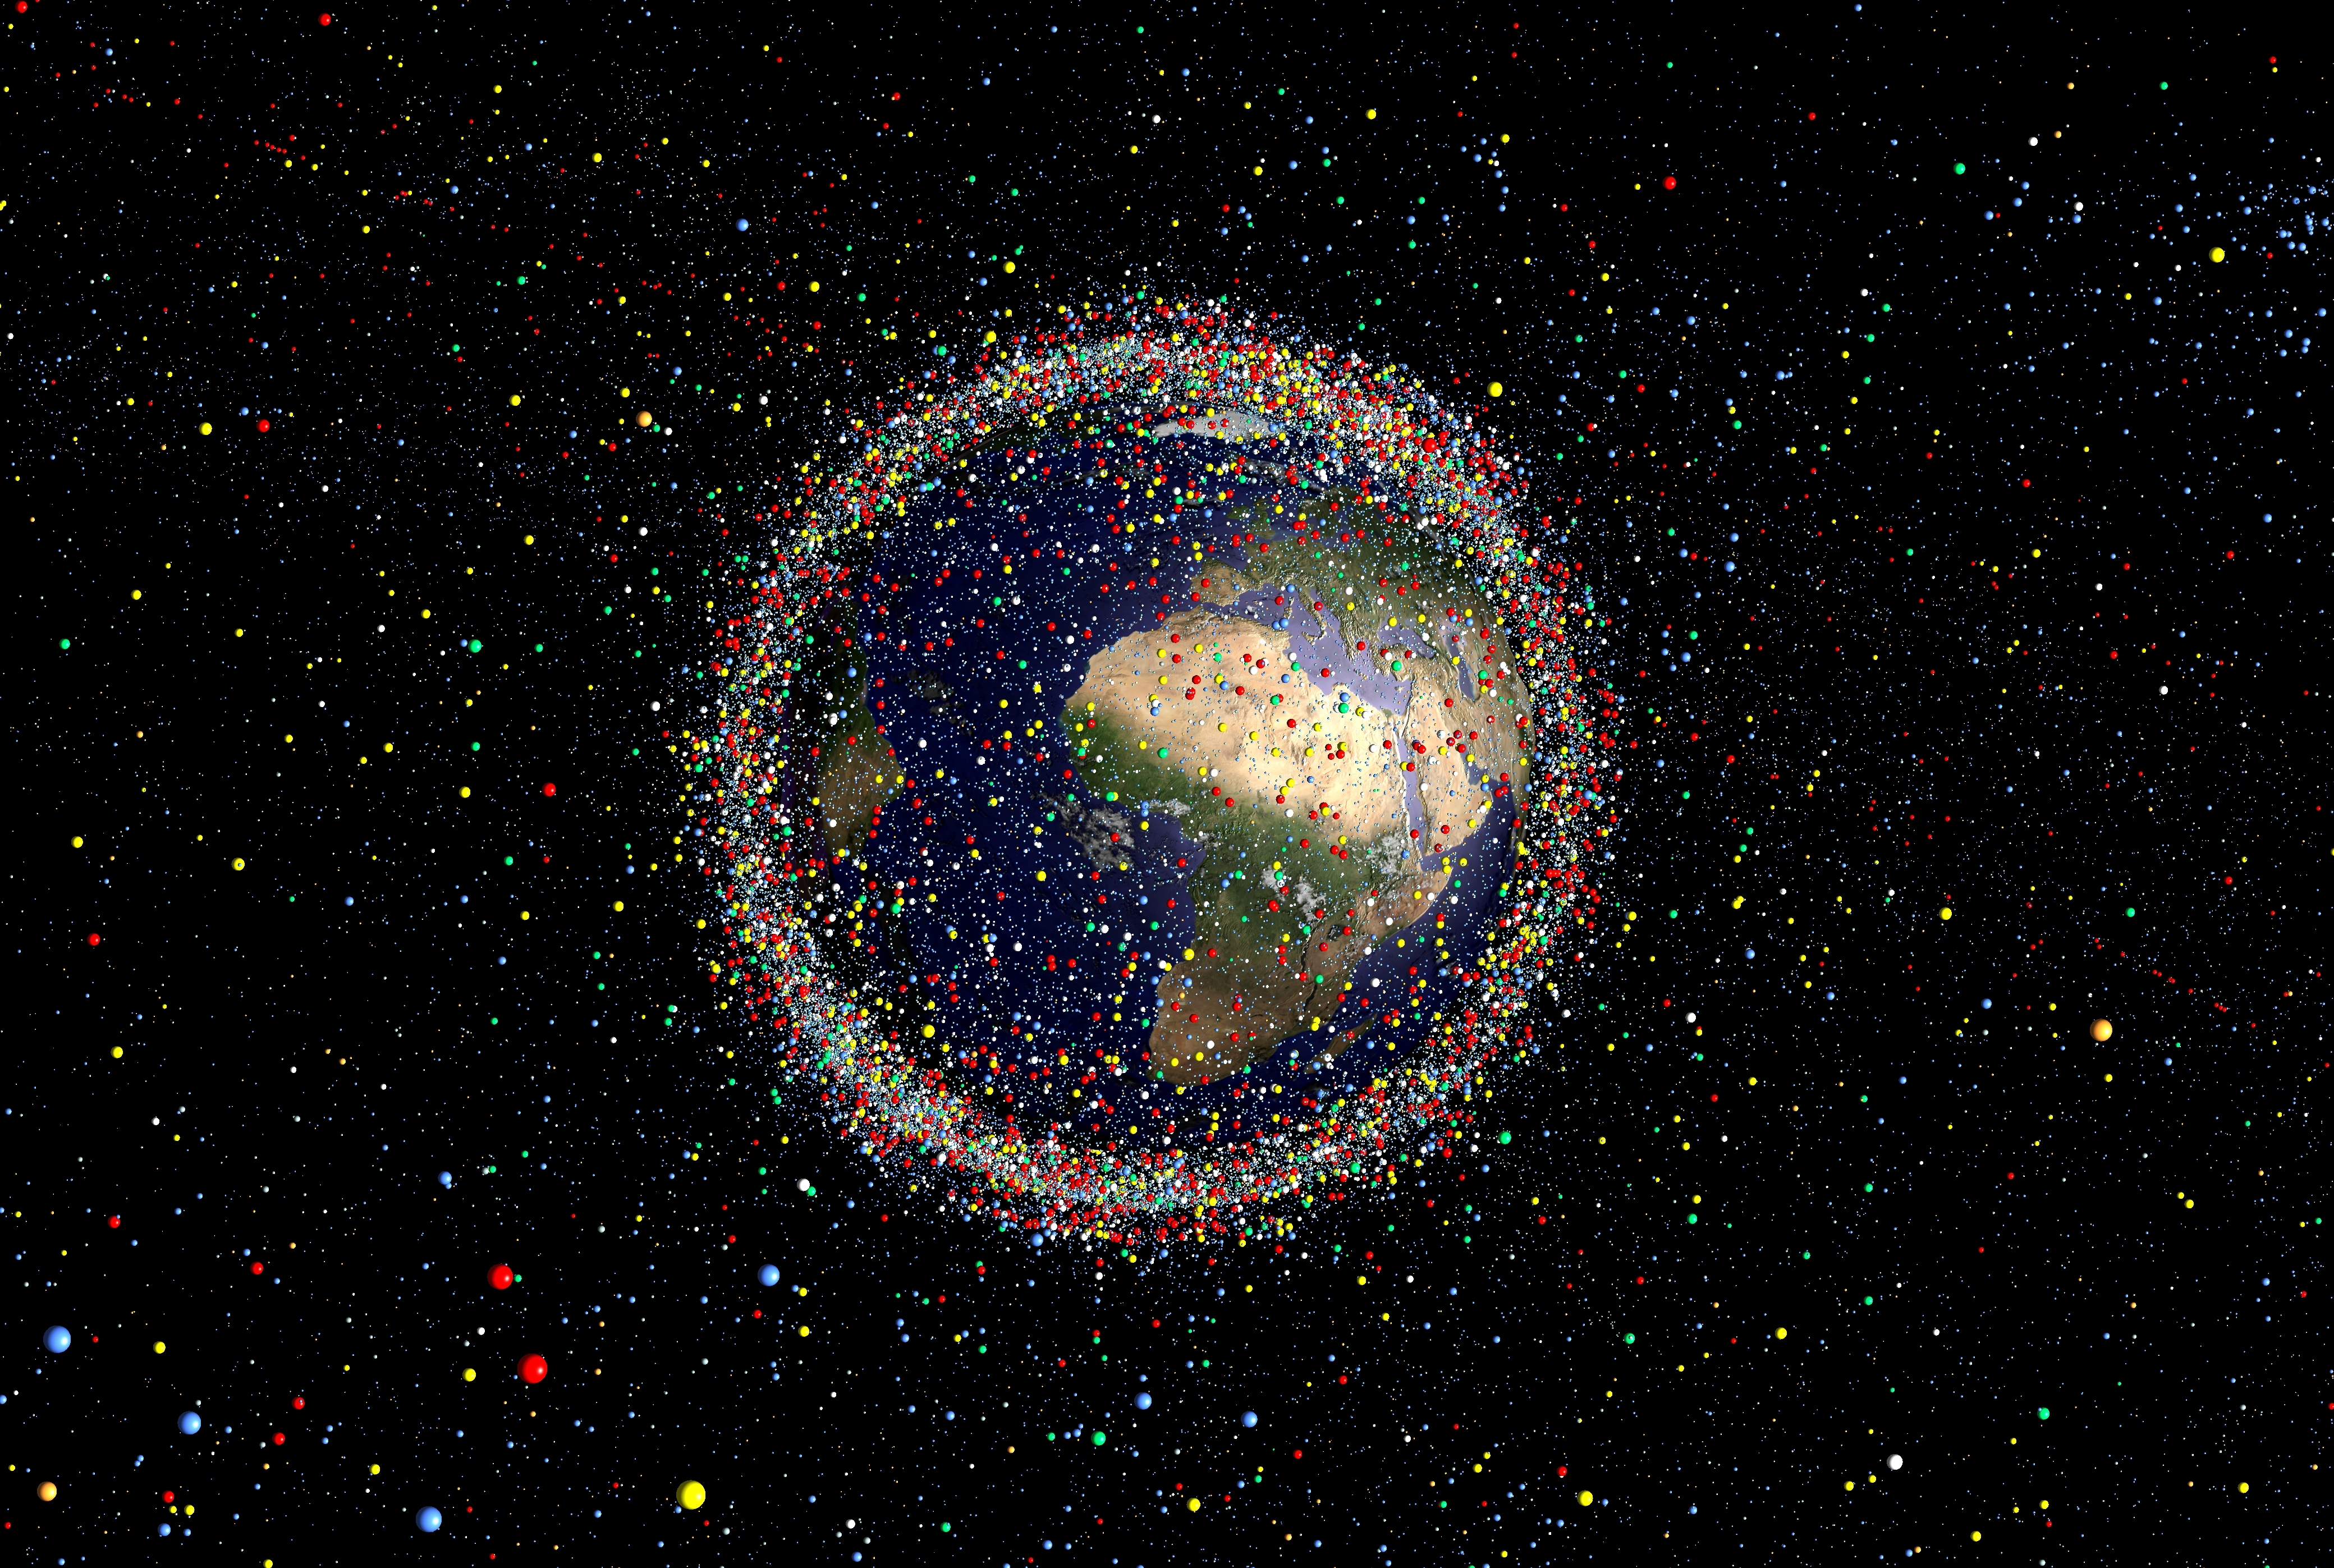
\includegraphics[scale=0.1]{./sections/Constellation_Deployment/S6-End_Of_Life/Images_S6/Picture_1_S6.jpg} 
\caption{View of the Space Debris around the Earth}
\end{figure}
\newline
\newline
The category that concerns the project is the non-functional spacecraft because it refers to all intact structures which have completed their mission. It is noticed that once satellite’s operative lifetime arrives to its end, the satellites stop maneuvering and counteracting perturbations to maintain the current orbit. Consequently, they tend to deviate from their nominal orbital parameters, starting an unknown trajectory and important repercussions. 
\newline
\newline
Therefore, by increasing the number of uncontrolled \textit{``dead''} satellites the probability of collision between working satellites and space debris increases at LEO as it is overcrowded. Space debris is small usually and its location can be followed from earth but is impossible to control it. Meanwhile, it is essential for space assets to be free of any impact because avoidance maneuvers are too complicated to have real success.  Thereby, the increasing risk of collision becomes the big threat everyone is fighting against. 

\subsection{End-of-Life Types and Analysis}

End-of-life strategies where implemented taking into account three factors: the time the satellite can orbit, the technical feasibility of active de-orbiting in terms of propellant and sub-systems enhancements and the altitude of its nominal orbital plane. 
\newline
\newline
The first one is related to the fact that the current recommendations say that any space asset that can become a non-functional spacecraft must de-orbit and disintegrate at its twenty-fifth birth on orbit. The second refers to the magnitude of the maneuver that can be developed with the power the thruster system can achieve. The third one is relevant because perturbations in space change according to the distance to the Earth’s surface. The closer it is the more perturbations from Earth and drag forces from the atmosphere the satellite suffers and perturbations help to de-orbit and disintegrate space assets.
\newline
\newline
Based on these premises, two different end-of-life groups had been determined: 

\begin{itemize}

\item[-] \textsc{Controlled de-orbit:}

It consists on carrying out a maneuver that leads to steep, controlled re-entry and burn-up in the atmosphere or ground impact. It must be done in a relatively short period of time, usually 1 revolution and it involves significantly high $\Delta V$. This sophisticated maneuver is initiated by a large increment of potential energy to make change the orbital altitude to a lower one well into the atmosphere where the satellite burns. A few calculations are useful to have a numerical result of that  $\Delta V$:
The velocity in the initial orbit is: 
\newline
\begin{center}
$V1 = \sqrt{\frac{GM_t}{R_t\,+\,h}}  = 7593.4 m/s$
\newline
\end{center}
Then the semi major axis of the elliptical orbit is obtained: 
\newline
\begin{center}
$a = {\frac{r1+r2}{2}} = 6672 km$
\newline
\end{center}
The speed at apogee of the elliptical orbit is: 
\newline
\begin{center}
$V2 = \sqrt{GM_t(\frac{2}{r}-\frac{1}{a})} = 7455 m/s$
\newline
\end{center}
Finally, the $\Delta V$ is computed: 
\newline
\begin{center}
$\Delta V = V1-V2 = 138.4 m/s$
\end{center}

\item[-]  \textsc{Uncontrolled de-orbit:}

A simpler and cheaper way to de-orbit satellites is to induce a reduction of the orbit altitude in order to cause a decay and ,finally, a re-entry to the atmosphere. The process is initiated by one or several arc maneuvers at apogee passes and it is carried out without controlling the trajectory. This procedure is appropriate for low-thrust systems and small satellites. 
\newline
In addition, when considering satellites placed at LEOs, this strategy takes advantages of the perturbations present in this altitudes (atmospheric drag). This force contributes to the decay increasing the rate of approach to the atmosphere. 

\end{itemize}